% !TeX root=../main.tex
\chapter{نتایج}
%\thispagestyle{empty} 
\label{chap:results}
\section{مقدمه} 
در این فصل ابتدا ملاحظات پیاده‌سازی روش پیشنهادی بیان می‌شود. سپس معیارهای ارزیابی که در پژوهش‌های مرتبط در این حوزه برای توصیف میزان دقت شبکه وجود دارد تعریف می‌گردد. و در ادامه ابتدا هر قسمت از روش‌های پیشنهادی شامل عملگر
\lr{LBP}
قابل آموزش، تابع هزینه 
\lr{ARCB}
و تابع هزینه‌ی مبتنی بر شناسه‌ی اشخاص روی یک دیتاست کوچک اجرا می‌گردد تا میزان تأثیر هر روش به تنهایی مشخص گردد. در انتها از تمام روش پیشنهادی برای دیتاست‌های بزرگ‌تر استفاده شده و دقت‌های به‌دست آمده با دقت برخی از معروف‌ترین روش‌های موجود در این حوزه مقایسه شود.
\section{ملاحظات پیاده‌سازی}
در این پایان‌نامه از زبان برنامه‌نویسی پایتون و کتابخانه
 \lr{Pytorch} \LTRfootnote{\href{https://pytorch.org}{https://pytorch.org}}
 استفاده شده است. این کتابخانه ابزاری قدرتمند برای مدل‌سازی شبکه‌های عمیق است. از آنجا که \lr{Pytorch} انعطاف‌پذیری بیشتری نسبت به ابزارهای مشابه دارد، پیاده‌سازی توابع جدید و عملگرهای غیر متداول در آن راحت‌تر است. در این پایان‌نامه یک عملگر جدید \lr{LBP} و تابع هزینه‌ی خاصی معرفی شده است که مشابه آن در ابزارهای یادگیری عمیق به‌صورت ماژول آماده وجود ندارد؛ اما توسط جریان محاسباتی \lr{Pytorch} قابل پیاده سازی است. 
\subsection{پیاده سازی \lr{LBP} قابل آموزش}
برای پیاده‌سازی یک عملگر جدید که دارای پارامتر قابل یادگیری باشد لازم است که یک کلاس با ارث‌بری از \lr{nn.Module} نوشته شود. با این‌کار این کلاس دارای قابلیت \lr{forward} و \lr{backward} خواهد بود و قابل استفاده در جریان محاسباتی شبکه عمیق خواهد بود.
برای آنکه این کلاس دارای پارامترهای یادگیرنده باشد لازم است که متغیر پارامترهای کلاس با استفاده از \lr{nn.Parameter} نوشته شود. با این کار در صورت استفاده از این عملگر به‌عنوان یک لایه در شبکه، پارامترهای عملگر \lr{LBP} در میان پارامترهای شبکه قرار می‌گیرند و بهینه‌سازی، منجر به به‌روزرسانی این پارامترها در کنار سایر پارامتر‌های شبکه به صورت خودکار خواهد شد.
\subsection{پیاده‌سازی تابع هزینه}
در هر بار \lr{forward} داده‌ها به شبکه پس از بلوک استخراج ویژگی یک بردار به‌دست خواهد آمد که لازم است این بردار در هر مرحله برای استفاده در دو تابع هزینه معرفی شده نرمالایز شوند. در حین تست شبکه از آنجا که تغییری در وزن‌ها رخ نخواهد داد یک بار نرمالایز کردن کافی خواهد بود. پیاده‌سازی تابع \lr{َARCB} با استفاده از توابع \lr{Pytorch} برای پایدار بودن محاسبات انجام شده است. پارامتر 
$s$
در تابع هزینه
\lr{ARCB}
در رابطه 
\ref{eq:arcb}
برابر با 64 در نظر گرفته شده است. مقادیر 
$\lambda_1$
و
$\lambda_2$
 در رابطه 
\ref{eq:ltot}
 هر کدام برابر با 
5.0
 در نظر گرفته شده‌اند.
 به‌منظور جلوگیری از بیش برازش داده‌ها از \lr{drop out}
\cite{srivastava2014dropout}
در لایه آخر پس از نرمالایز کردن بردار ویژگی و پیش از طبقه‌بند استفاده شده است. 
برای پیاده سازی تابع هزینه مبتنی بر شناسه اشخاص نیاز است به غیر از تصویر ورودی و برچسب تصویر، یک عدد به‌عنوان شناسه نیز در اختیار باشد. در دیتاست‌های موجود یافتن عدد شناسه از روی نام فایل ویدئو قابل تشخیص است. برای بهینه‌سازی شبکه از الگوریتم آدام 
\cite{kingma2014adam}
استفاده شده است.
\subsection{بارگذاری داده‌ها برای آموزش}
برای بارگذاری و آماده‌سازی داده‌ها، توابع و کلاس‌های آماده در کتابخانه \lr{Pythoch} وجود دارد که به‌صورت خودکار تصاویر موجود در یک پوشه استفاده خواهد کرد اما به‌دلیل ماهیت ویدیویی داده‌ها و همچنین تابع هزینه خاص معرفی شده نمی‌توان از توابع آماده استفاده کرد.
در برخی دیتاست‌ها فایلی برای مختصات چهره وجود دارد که می‌توان در هر فریم ویدیو، قسمت مربوط به چهره را برش زد و به‌جای استفاده از کل فریم تنها قسمت چهره به همراه کمی از قسمت پس‌زمینه تصویر به‌عنوان ورودی به شبکه داده شود. در دیتاست‌هایی که این فایل مختصات وجود ندارد با استفاده از روش \lr{MTCCN}
\cite{zhang2016joint}
 چهره فریم‌ها پیدا شده و در یک فایل متنی ذخیره شده است.
 
دیتاست‌های معرفی شده همگی به‌صورت ویدیو هستند. از آنجا که روش ارائه شده روی تک تصویر کار می‌کند یکی از نکات عملی در خصوص آموزش روی داده‌های ویدیویی، نحوه آماده‌سازی داده‌ها برای آموزش است. یک روش تبدیل ویدیو به تصویر و ذخیره آن روی دیسک است. اما این کار موجب مصرف شده حجم زیادی از دیسک خواهد شد و از آنجا که در حین آموزش لازم است که تصاویر مجدداً از دیسک به حافظه \lr{RAM} بارگذاری شوند روال آموزش کند خواهد شد.
از طرفی از آنجا که نمونه‌های موجود در دو کلاس با یک دیگر برابر نیستند به‌منظور پایدار شدن تابع هزینه \lr{ARCB} لازم است که در هر دسته به تعداد نزدیک هم تصویر از هر کلاس وجود داشته باشد. از طرفی برای آنکه تابع هزینه مبتنی بر شناسه اشخاص به‌درستی عمل کند لازم است که پراکندگی تصاویر در هر دسته به‌اندازه کافی باشد تا حالت‌های مختلف از اشخاص با شناسه‌های متفاوت و برچسب متفاوت در دسته وجود داشته باشد. همچنین لازم است که ترتیب داده‌ها تا حد ممکن تصادفی باشند تا غیر یقینی بیشتری در حین آموزش، برای شبکه وجود داشته باشد. 

در پیاده‌سازی روش این پایان‌نامه ابتدا به تعداد دسته، ویدیو در حافظه \lr{RAM} بارگذاری خواهد شد و در هر مرحله یک فریم به‌صورت تصادفی از هر ویدیو انتخاب می‌شود که در نهایت به تعداد دسته، فریم برای آموزش وجود خواهد داشت. با این کار این فریم‌ها هر کدام از ویدیوهای متفاوتی هستند که موجب می‌شود تصاویر موجود در دسته پراکندگی لازم را داشته باشند. در مراحل بعدی از همین ویدیوها که در حافظه \lr{RAM} بارگذاری شده‌اند استفاده خواهد شد و این روال تا زمانی که فریم در ویدیوها وجود داشته باشد ادامه خواهد داشت. سپس دسته ویدئو دیگری انتخاب خواهد شد و آموزش روی همه ویدیوها ادامه دارد. 

از آنجا که پس از انتخاب تعدادی ویدیو، به تعداد فریم‌های آن و به‌صورت متوالی مرحله‌های آموزش تکرار می‌شود و فریم‌های متوالی یک ویدئو از نظر ظاهری نزدیک به هم هستند لازم است که غیر یقینی داده‌ها بیشتر شود بدین منظور از روش‌های افزایش داده 
\LTRfootnote{Data augmentation}
به‌صورت تصادفی استفاده می‌شود. بدین منظور از تبدیلاتی که هر تصویر ورودی را به‌صورت تصادفی چرخش می‌دهند استفاده می‌شود. 

به‌منظور جلوگیری از بیش برازش از روش پاک کردن تصادفی قسمتی از تصویر ورودی استفاده شده است 
\cite{zhong2020random}
. همچنین هنگامی که قرار است قسمت چهره به همراه پس زمینه برش زده شود این کار به‌صورت یک پنجره تصادفی انجام می‌شود؛ بدین ترتیب در هر بار بارگذاری داده‌ها موقعیت چهره در تصویر برش زده تصادفی خواهد بود و لزوماً همیشه در مرکز تصویر نخواهد بود.
در شکل  
\ref{fig:aug}
نحوه برش زدن تصادفی چهره به همراه پس زمینه نشان داده شده است. در این تصویر مستطیل آبی چهره فرد را نشان می‌دهد و مستطیل‌های رنگی به‌صورت تصادفی برای هر بار انتخاب چهره انتخاب می‌شوند. و در انتها تصویر انتخابی به 224*224 تغییر اندازه می‌شود.
\begin{figure}[ht]
	\centerline{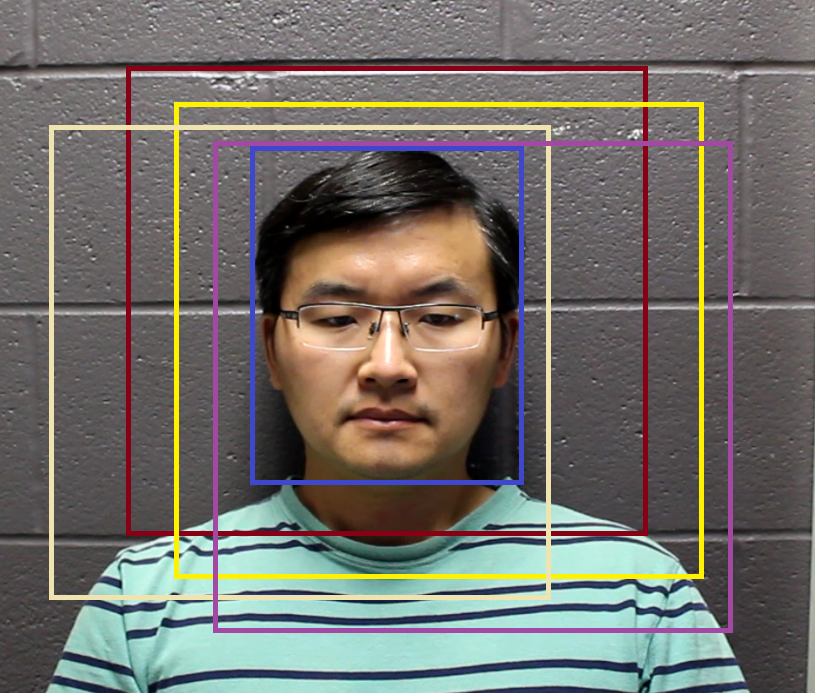
\includegraphics[width=0.7\linewidth]{aug}}
	\caption{نحوه برش زدن تصادفی چهره با مقداری از پس‌زمینه}
	\label{fig:aug}
\end{figure}

برای پیاده سازی کلاس بارگذاری داده یک
 \lr{Data loader} 
سفارشی نوشته شده است و همچنین برای آنکه استراتژی ترتیب تصادفی انتخاب ویدیو و استفاده مجدد از فریم‌های ویدیو متوالی پیاده شود یک تابع \lr{Batch sampler} سفارشی نوشته شده است. در پیاده‌سازی این تابع از مفهوم \lr{Iteration} در زبان برنامه‌نویسی پایتون استفاده شده است.
\section{معیارهای ارزیابی}
مسئله کشف تقلب یک مسئله طبقه‌بندی دو کلاسه است که در هنگام آزمون، معمولاً تعداد نمونه‌های واقعی و تقلبی یکسان نیستند. به همین دلیل معیار دقت شبکه یعنی تعداد نمونه‌های درست پیش‌بینی شده تقسیم بر تعداد کل نمونه‌ها ملاک خوبی برای قضاوت در مورد عملکرد شبکه نیست. 

بدین منظور از معیاری به نام نرخ خطای برابر 
\LTRfootnote{Equal Error Rate} ($EER$)
و ترسیم آن به ازای آستانه‌های مختلف، در قالب نمودار نرخ خطای برابر استفاده می‌شود. 
دو حالت برای تشکیل این نمودار مهم است. نرخ خطای قبول کردن
\LTRfootnote{False acceptance rate} ($FAR$)
 نمونه، که به معنی این است که برچسب واقعی چهره زنده بوده است اما به‌عنوان چهره تقلبی پیش‌بینی شده است. و نرخ خطای رد کردن
 \LTRfootnote{False rejection rate} ($FRR$)
  که به معنی این است که نمونه برچسب تقلبی دارد ولی به‌عنوان چهره زنده پیش‌بینی شده است.
\begin{equation} \label{eq:far}
	FAR = \frac{number\; of\; false\; accepted\; samples}{total\; number\; of\; fake\; samples}
\end{equation}
\begin{equation} \label{eq:frr}
	FAR = \frac{number\; of\; false\; rejected\; samples}{total\; number\; of\; real\; samples}
\end{equation}

معمولاً این مقدار بر اساس یک آستانه که یک پارامتر است محاسبه می‌گردد. برای مثال در شبکه‌ی عصبی مقدار تک نورون لایه آخر با تابع فعالسازی سیگموید، مقداری بین صفر و یک خواهد داشت. و با انتخاب یک سطح آستانه و مقایسه مقدار نورون لایه‌ی آخر با این سطح آستانه تصمیم‌گیری در مورد پیش‌بینی برچسب نمونه انجام می‌شود. نرخ خطای برابر، برابر با مقداری است که $FAR$ با $FRR$ برابر شود.

\begin{equation}\label{eq:taueer}
	\tau_{EER} = \argmin_{\tau}|FAR(\tau)-FRR(\tau)|
\end{equation}
\begin{equation}\label{eq:eer}
	EER=FAR(\tau_{EER})=FRR(\tau_{EER})
\end{equation}

در شکل
\ref{fig:eer}
این معیار را در قالب نمودار به ازای سطوح مختلف آستانه نشان می‌دهد. در دیتاست‌هایی که داده دارای سه قسمت آموزش، توسعه و آزمون است، معمولاً روی داده‌های آموزش وزن‌های شبکه به‌دست می‌آید و روی قسمت توسعه، پارامتر  
$\tau_{EER}$
 به دست خواهد آمد. و روی قسمت آزمون معیار نصف کل نرخ خطا
\LTRfootnote{Half total error rates}
  به‌صورت رابطه
\ref{eq:hter}
تعریف می‌شود.

\begin{equation}\label{eq:hter}
	HTER=\frac{FAR(\tau_{EER})+FRR(\tau_{EER})}{2}
\end{equation}

 \begin{figure}[ht]
	\centerline{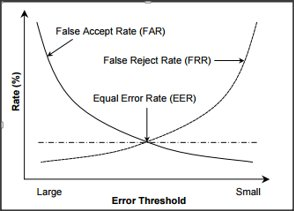
\includegraphics[width=0.5\linewidth]{eer}}
	\caption{نمودار میزان خطای برابر}
	\label{fig:eer}
\end{figure}

با تحلیل نمودار نرخ خطای برابر، می‌توان در مورد میزان عملکرد شبکه بحث کرد. هر چه که مقدار تقاطع منحنی $FRR$ و
$FAR$

پایین‌تر باشد، شبکه دقت بهتری دارد. همچنین مقدار
 $FRR$ و $FAR$
در نزدیکی‌های محل تقاطع نشان می‌دهد که شبکه چه میزان دو کلاس را از هم جدا کرده است. این یعنی نه تنها مقدار نرخ خطای برابر اهمیت دارد بلکه مطلوب این است که با تغییرات جزئی میزان سطح آستانه، نرخ خطا در اطراف آن نیز کم باشد. هر چه مقدار خطا در اطراف محل تقاطع دو منحنی کوچکتر باشد شبکه قابلیت تعمیم‌پذیری بیشتری روی داده‌های دیده نشده خواهد داشت.

یک معیار دیگر برای ارزیابی استفاده از استاندارد
 \lr{ISO/IEC 30107-3} 
است که در آن از نرخ خطای طبقه‌بندی ارائه حمله
\LTRfootnote{Attack Presentation Classification Error Rate}  ($APCER$) 
و نرخ خطای طبقه بندی ارائه خوب
\LTRfootnote{Bona Fide Presentation Classification Error Rate} ($BPCER$) 
تعریف می‌شود که در آن
$BPCER$
 معادل
$FRR$ 
است ولی
$APCE$
معادل بیشترین
$FAR$ 
به ازای ابزارهای حمله مختلف است.
منظور از ابزار حمله، حمله کاغذ چاپ‌شده یا حمله بازپخش است. رابطه 
\ref{eq:apcer}
نحوه محاسبه 
$APCER$
را نشان می‌دهد که در آن 
$PAI$
معادل ابزار حمله ارائه
\LTRfootnote{Presentation Attack Instrument}
است. در دیتاست‌های مورد استفاده در این پایان‌نامه 
$PAI$
پارامتر دو مقدار خواهد داشت که یکی برای حمله کاغذ چاپ‌شده و دیگری برای حمله بازپخش است.
همچنین متوسط نرخ خطای طبقه‌بندی 
\LTRfootnote{Average Classification Error Rate} $APCER$
به‌صورت میانگین 
$APCER$
 و 
$BPCER$ 
تعریف می‌شود.
\begin{equation}\label{eq:apcer}
	APCER=\max_{PAI=1,...,C}{FAR_{PAI}}
\end{equation}
\begin{equation}\label{eq:ACER}
	ACER=\frac{APCER+BPCER}{2}
\end{equation}
\section{عملکرد مدل در دیتاست‌ها}
این بخش به بررسی دقت روش پیشنهادی روی دیتاست‌های مختلف می‌پردازد. در ابتدا برای بررسی اثر بخشی روش پیشنهادی روی دیتاست \lr{Replay} که دیتاست نسبتاً کوچکی است، روش پیشنهادی بررسی می‌شود. این کار با هدف اثبات مفهوم
\LTRfootnote{Proof of concept}
 انجام می‌شود. و سپس روی دیتاست‌های دیگر دقت گزارش می‌شود.
\subsection{اثر عملگر \lr{LBP} قابل آموزش در دیتاست \lr{Replay}}
به‌منظور مقایسه‌ی روش‌های پیشنهادی و تأثیر آنها در بهبود دقت ابتدا یک شبکه \lr{ALEXNET} بدون عملگر \lr{LBP} با تابع هزینه \lr{BCE} به کار برده می‌شود. نمودار نرخ خطای برابر، برای این مورد به‌صورت شکل 
\ref{fig:eer-alex-bce} 
است. 
\begin{figure}[h]
	\centerline{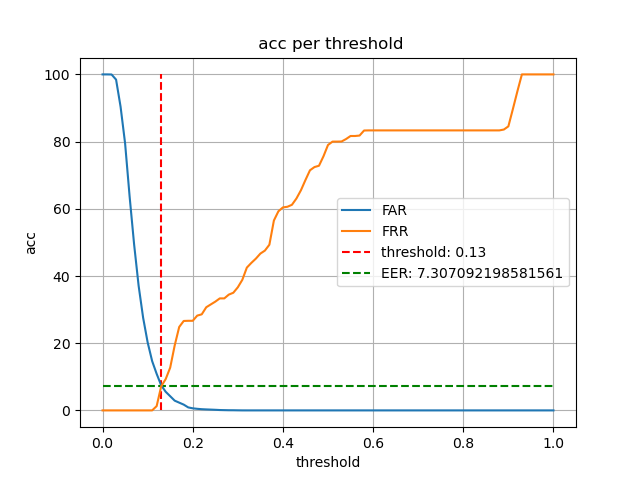
\includegraphics[width=0.65\linewidth]{eer-alex-bce}}
	\caption{نمودار خطای برابر برای شبکه \lr{ALEXNET} و تابع هزینه \lr{BCE}}
	\label{fig:eer-alex-bce}
\end{figure}

همانطور که مشاهده می‌شود با سطح آستانه متناظر با محل تقاطع دو نمودار برابر  
$\tau_{EER} = 0.13$
برای نورون آخر است که در این سطح آستانه نرخ خطای برابر  
$EER = 7.3 \%$
 روی داده دیده نشده به دست می‌آید. اما لازم است توجه شود تنها مقدار خطا مهم نیست و عملکرد نمودار در سایر مقادیر سطح آستانه نیز مهم است و در سطح آستانه 
 $\tau = 0.6$
  مقدار خطا 
$FRR=80\%$  
   است که بسیار زیاد است. هر چند که در این ناحیه خطا
  $FAR =0$
است. این تفاوت بین دو مقدار خطا نشان می‌دهد که دو کلاس  از یک دیگر جدا نشده اند و استخراج ویژگی به درستی صورت نگرفته است. همچنین در اطراف سطح آستانه 
  $\tau_{EER} = 0.13$
  با کمی تغییر در سطح آستانه مقدار خطا بزرگ می‌شود.


با استفاده از عملگر \lr{LBP} قابل آموزش پیش از \lr{ALEXNET} و تابع هزینه نیز کماکان \lr{BCE} باشد نمودار شکل
\ref{fig:eer-lbp}
به‌دست می‌آید.
\begin{figure}[h]
	\centerline{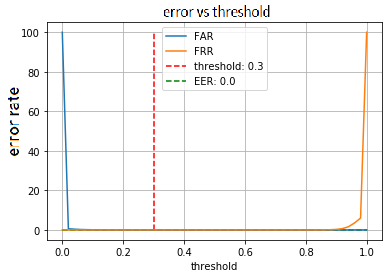
\includegraphics[width=0.65\linewidth]{eer-lbp}}
	\caption{نمودار خطای برابر هنگام استفاده از عملگر \lr{LBP} پیشنهادی}
	\label{fig:eer-lbp}
\end{figure}
همانطور که مشاهده می‌شود استفاده از تنها یک لایه 
\lr{LBP}
 پیش از \lr{ALEXNET} مقدار خطا را به صفر درصد رسانده است. همچنین وضعیت خطا در اطراف آستانه نیز بهبود یافته است.
از آنجا که افزودن یک لایه عملگر \lr{LBP} قابل آموزش، بار محاسباتی به شبکه اضافه می‌کند برای مقایسه دیگر نمودار آموزش شبکه با تابع هزینه \lr{BCE} و شبکه
 \lr{EfficientNet B0} 
با شروع از وزن‌های تصادفی، به صورت شکل 
\ref{fig:eer-eff}
است.
\begin{figure}[h]
	\centerline{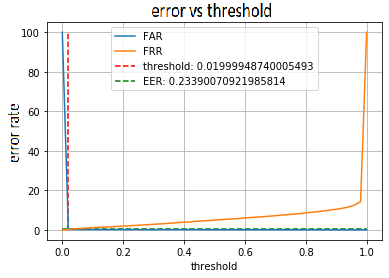
\includegraphics[width=0.65\linewidth]{eer-eff}}
	\caption{نمودار خطای برابر هنگام استفاده از شبکه \lr{EfficientNet B0}}
	\label{fig:eer-eff}
\end{figure}

این نمودار نشان می‌دهد لزوماً استفاده از شبکه پیچیده نمی‌تواند به نتیجه مطلوب برساند. 
لازم است توجه شود این نمودار بدین معنی نیست که لایه \lr{LBP} به همراه \lr{ALEXNET} قدرت بیشتری نسبت به شبکه \lr{Efficient net} دارد. بلکه در این کاربرد خاص و دیتاست \lr{Replay} که حجم داده کمی دارد استفاده از شبکه ساده‌تر اما هوشمندانه با توجه به مسئله، دقت بهتری را ایجاد می‌کند.
\subsection{اثر تابع هزینه \lr{ARCB} در دیتاست \lr{Replay}}
اکنون تنها از شبکه \lr{ALEXNET} بدون عملگر \lr{LBP} استفاده می‌شود ولی تابع هزینه \lr{ARCB} معرفی شده به‌جای تابع \lr{BCE} استفاده می‌شود. نمودار شکل
\ref{fig:eer-arcb}
نشان می‌دهد تغییر تابع هزینه بدون تغییری در ساختار می‌تواند تاثیرگذار باشد. نمودار در مقایسه با نمودارهای قبلی متقارن‌تر شده است .در این شکل میزان خطا در اطراف سطح آستانه صفر است ولی با دور شدن از سطح آستانه و نزدیک شدن به مقدار 0 و 1 خطا بیشتر می‌شود. این تأثیر حاشیه در تابع هزینه \lr{ARCB} است که موجب شده است دو کلاس با یک حاشیه از یک دیگر جدا شوند. در این حالت اگر مقدار آستانه در اطراف 
$\tau_{EER} = 0.67$
و در بازه 
$ 0.39\le \tau \le 0.75$
قرار داشته باشد مقدار خطا
 $FRR$ و $FAR$
 هر دو صفر خواهد بود. این باند اطمینان حاصل افزودن 
 $m$
در رابطه تابع هزینه
\lr{ARCB}
است که موجب جداسازی دو کلاس شده است. همچنین این تابع هزینه در مقایسه با تابع هزینه
\lr{BCE}
میزان خطای برابر را نیز کاهش داده است که بدین معناست که تابع هزینه، شبکه استخراج ویژگی را مجبور کرده است که به دنبال ویژگی‌های اساسی برای جداسازی دو کلاس با حاشیه باشد.
\begin{figure}[h]
	\centerline{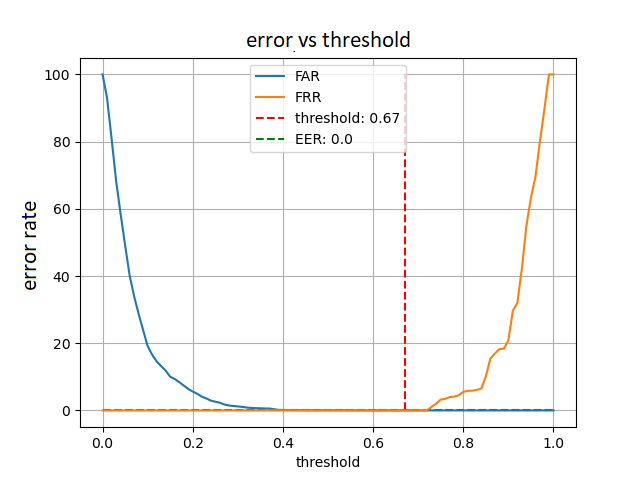
\includegraphics[width=0.65\linewidth]{eer-arcb}}
	\caption{نمودار خطای برابر هنگام استفاده از تابع هزینه \lr{ARCB} پیشنهادی}
	\label{fig:eer-arcb}
\end{figure}

\subsection{اثر تابع هزینه بر پایه شناسه‌ی اشخاص در دیتاست \lr{Replay}}
اکنون از ساختار ساده \lr{ALEXNET} استفاده می‌شود و تابع هزینه برای طبقه‌بند تابع \lr{BCE} است ولی تابع هزینه مبتنی بر شناسه اشخاص نیز به آن افزوده شده‌است. نمودار این حالت به‌صورت شکل 
\ref{fig:eer-pid}
است. همانطور که مشاهده می‌شود خطا در آستانه‌های 
$ 0.01\le \tau \le 0.8$
به‌صورت مطلق صفر است. این خطای صفر در این باند آستانه، نشان دهنده تاثیر تابع هزینه مبتنی بر شناسه اشخاص است. با به کار بردن این تابع هزینه و بدون هیچ تغییری در ساختار شبکه، وزن‌های شبکه به گونه‌ای تغییر یافته‌اند که ویژگی‌های اساسی مربوط به تقلب را پیدا کنند و به ویژگی‌های ظاهری چهره افراد توجه نکنند. 
\begin{equation}\label{eq:pid2}
	L_{PiD} = \sum_{l_1 \ne l_2,k_1 \ne k_2}{\frac{1}{N_i}d( X_{k_1}^{l},X_{k_2}^{l})+\frac{1}{N_j}\max(0,M-d( X_{k}^{l_1},X_{k}^{l_2} ))}
\end{equation}
چنان که در رابطه 
\ref{eq:pid2}
مشاهده می‌شود  عبارت اول این تابع هزینه باعث می‌شود جفت نمونه‌های دارای یک برچسب و شناسه شخص متفاوت به یک‌دیگر نزدیک‌تر شوند و در عبارت دوم جفت نمونه‌های یک شخص و متعلق به کلاس‌های متفاوت از یک‌دیگر به مقدار ‌
$M$
در فضای نرمالایز شده دور شوند.
\begin{figure}[!h]
	\centerline{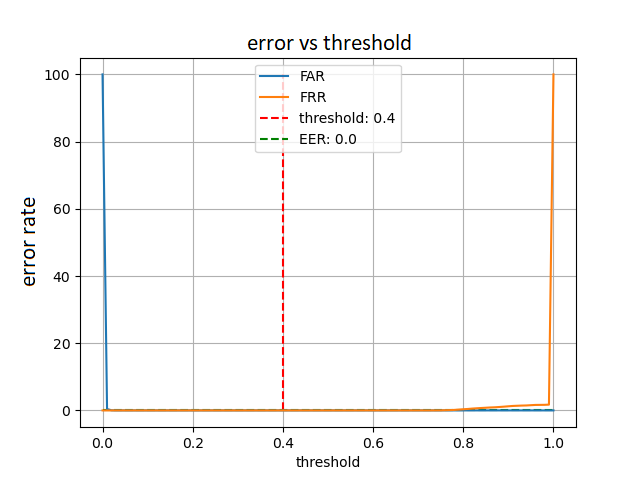
\includegraphics[width=0.65\linewidth]{eer-pid}}
	\caption{نمودار خطای برابر با استفاده از تابع هزینه مبتنی بر شناسه اشخاص}
	\label{fig:eer-pid}
\end{figure}

تا این قسمت اثر هر کدام از روش‌های پیشنهادی به تنهایی بررسی شده‌اند. برای ادامه فصل تمامی روش‌ها در کنار یک‌دیگر استفاده می‌شود. و شبکه استخراج ویژگی
\lr{EfficientNet B0} 
است. همچنین به‌منظور تسریع در همگرا شدن شبکه، قسمت استخراج ویژگی از وزن‌های آموزش دیده روی دیتاست
 \lr{ImageNet} \cite{deng2009imagenet}
استفاده می‌شود ولی این وزن‌ها حین آموزش تغییر می‌کند.


\subsection{نتایج روی دیتاست‌های \lr{CASIA} و \lr{MSU}}
دیتاست‌های \lr{MSU} و \lr{CASIA} نسبت به دیتاست \lr{Replay} دارای رزولوشن تصویر بیشتری هستند. این دیتاست‌ها بر خلاف دیتاست \lr{replay} که دارای سه قسمت آموزش، توسعه و آزمون است تنها دارای دو قسمت آموزش و آزمون می‌باشد. در جدول
\ref{tab:eercasiamsu}
 مقدار نرخ خطای برابر در قسمت آزمون دیتاست گزارش شده است.
\begin{table}[!h]
	\caption{خطای برابر روی دیتاست‌های \lr{CASI‌A} و ‌\lr{MSU}}
	\label{tab:eercasiamsu}
	\centering
	\onehalfspacing
	\begin{tabular}{|c|c|}
		\hline \lr{Dataset} &\lr{ EER (\%)}   \\
		\hline \lr{CASIA}   & \lr{0.54}     \\
		\hline \lr{MSU}     & \lr{0.0} \\
		   \hline
	\end{tabular} 
\end{table}

از آنجا که این دو دیتاست کمی قدیمی هستند رسیدن به نرخ خطای صفر چندان دشوار نیست. در پژوهش‌های اخیر در این حوزه، عمده گزارش‌های دقت روی دیتاست‌های \lr{SIW} و \lr{OULU} است. این دو دیتاست نسبت به دیتاست‌های قبلی جدیدتر و دارای حجم بیشتری هستند. به همین دلیل در پژوهش‌های اخیر بیشتر از این دو دیتاست استفاده شده است. هر کدام از این دو دیتاست دارای پروتکل‌های مختلفی هستند که حالت‌های مختلف برای بررسی تعمیم‌پذیری مدل را نشان می‌دهد.
\subsection{دقت در دیتاست \lr{SIW}}
در پروتکل اول دیتاست \lr{SIW} به بررسی تغییر حالت چهره می‌پردازد. بدین منظور برای آموزش از 60 فریم اول هر ویدیو استفاده می‌شود ولی برای آزمون از تمامی فریم‌های ویدیوهای تست استفاده می‌شود. از آنجا که در فریم­‌های ابتدایی هر ویدیو، کاربر صورت خود را تکان نمی‌دهد پس داده‌های آموزش تنها شامل تصاویر صورت با موقعیت ثابت در مقابل دوربین است. ولی داده‌های تست شامل همه حالت‌های حرکت چهره در ویدئو است. این پروتکل قابلیت تعمیم‌پذیری مدل ارائه شده را در حالت‌های مختلف چهره نشان می‌دهد. نتایج این حالت در جدول
\ref{tab:siw1}
همراه با مقایسه با برخی روش‌های معروف ذکر شده است.
\begin{table}[h]
	\caption{نرخ در پروتکل اول دیتاست \lr{SIW}}
	\label{tab:siw1}
	\centering
	\onehalfspacing
	\begin{tabular}{|c|c|c|l|}
	\hline \lr{ACER} & \lr{BPCER} & \lr{APCER} & \lr{Method}                \\
	\hline \lr{3.58} & \lr{3.58}  & \lr{3.58}  & \cite{liu2018learning} \lr{Auxiliary}    \\
	\hline \lr{0.25} & \lr{0.50}  & \lr{0}     & \cite{feng2020learning} \lr{LGSC}         \\
	\hline \lr{1}    & -     & -     & \cite{yang2019face} \lr{STASN}       \\
	\hline \lr{0.12} & \lr{0.17}  & \lr{0.07}  & \cite{yu2020searching} \lr{CDCN}             \\
	\hline \lr{0.4}  & \lr{0.17}  & \lr{0.64}  & \cite{wang2020deep} \lr{SGTD}      \\
	\hline \lr{0.4}  & \lr{0.17}  & \lr{0.69}  & \cite{li20203dpc}   \lr{3DPC-NET}   \\
	\hline \lr{0.13} & \lr{0.12}  & \lr{0.14}  & \lr{ARCB+PID}    \\ 
	 \hline         
	\end{tabular}
\end{table}

در پروتکل دوم از چهار نوع حمله‌ی بازپخش، هر بار یک حمله برای تست کنار گذاشته می‌شود و آموزش شبکه روی سه حمله‌ی بازپخش دیگر انجام می‌شود. پس برای این پروتکل چهار حالت مختلف وجود دارد که میانگین و واریانس دقت روی چهار حالت گزارش می‌شود. این پروتکل با هدف بررسی عمکرد روش پیشنهادی روی نوع حمله بازپخش دیده نشده طراحی شده است. نتایج در جدول 
\ref{tab:siw1}
گزارش شده است.
\begin{table}[!h]
	\caption{نرخ در پروتکل دوم دیتاست \lr{SIW}}
	\label{tab:siw2}
	\centering
	\onehalfspacing
	\begin{tabular}{|c|c|c|l|}
		\hline \lr{ACER}          & \lr{BPCER}       & \lr{APCER}         & \lr{Method}                  \\
		\hline \lr{0.57 ±0.69}    & \lr{0.57 ±0.69}  & \lr{0.57 ±0.69}    & \cite{liu2018learning} \lr{Auxiliary}     \\
		\hline \lr{0±0}           & \lr{0±0}         & \lr{0±0}           & \cite{feng2020learning} \lr{LGSC}           \\
		\hline \lr{0.28±0.05}     & -           & -             & \cite{yang2019face} \lr{STASN}           \\
		\hline \lr{0.04±0.5}      & \lr{0±0.09}      & \lr{0±0}           & \cite{yu2020searching} \lr{CDCN}            \\
		\hline \lr{0.02±0.04}     & \lr{0.04±0.08}   & \lr{0.0±0.0}       & \cite{wang2020deep} \lr{SGTD}        \\
		\hline \lr{0.45±0.14}     & \lr{0.43±0.06}   & \lr{0.46±0.28}     & \cite{li20203dpc}   \lr{3DPC-NET}   \\
		\hline \lr{0.0087±0.0151} & \lr{0.01±0.0173} & \lr{0.0075±0.0129} & \lr{ARCB+PID}                \\
		\hline         
	\end{tabular}
\end{table}

\subsection{دقت در دیتاست \lr{OULU}}
دیتاست \lr{OULU} نیز دارای چهار پروتکل مختلف است که در این پایان‌نامه دقت روی پروتکل اول و دوم گزارش شده است. 
دیتاست \lr{OULU} در سه مکان مختلف تصویر برداری شده است. در پروتکل اول روی ویدیوهای مربوط به مکان اول و دوم آموزش صورت می‌گیرد و در ویدیوهای مکان سوم آزمون انجام می‌گیرد. این پروتکل با این هدف ارائه شده است که قابلیت روش پیشنهادی با تغییر مکان تصویربرداری ارزیابی شود. نتایج به دست آمده به همراه مقایسه با روش‌هایی که روی این دیتاست روش خود را ارزیابی کرده‌اند در جدول
\ref{tab:oulu1}
گزارش شده است.
\begin{table}[h]
	\caption{دقت در پروتکل اول  دیتاست \lr{OULU}}
	\label{tab:oulu1}
	\centering
	\onehalfspacing	\begin{tabular}{|c|c|c|l|}
		\hline               
		\lr{ACER} & \lr{BPCER}          & \lr{APCER} & \lr{Method}                  \\
		\hline \lr{5.7}  & \lr{8.9}            & \lr{2.5}     & \cite{tu2020learning}\lr{GFA}  \\
		\hline \lr{1.6}  & \lr{1.6}            & \lr{1.6}      & \cite{liu2018learning} \lr{Auxiliary}  \\
		\hline \lr{1.5}  & \lr{1.7}            & \lr{1.2}      & \cite{jourabloo2018face} \lr{FaceDs}    \\
		\hline \lr{0.4}  & \lr{0}              & \lr{0.8}      & \cite{feng2020learning} \lr{LGSC}       \\
		\hline \lr{1.9}  & \lr{2.5}            & \lr{1.2}     & \cite{yang2019face} \lr{STASN}       \\
		\hline \lr{0.2}  & \lr{0}              & \lr{0.4}      & \cite{yu2020searching} \lr{CDCN}       \\
		\hline \lr{1.0}  & \lr{0.0}            & \lr{2.0}      & \cite{wang2020deep} \lr{SGTD}       \\
		\hline \lr{0.42} & \lr{0}              & \lr{0.83}    & \cite{george2019deep} \lr{DeepPixBis}\\
		\hline \lr{1.1}  & \lr{1.3}            & \lr{0.8}      & \cite{liu2020disentangling}\lr{STDN}     \\
		\hline \lr{1.2}  & \lr{0}              & \lr{2.3}     & \cite{li20203dpc}   \lr{3DPC-NET}   \\
		\hline \lr{2.29} & \lr{2}              & \lr{2.58}    & \lr{ARCB+PID} \\              
		\hline         
	\end{tabular}
\end{table}

در پروتکل دوم از دو حمله کاغذ چاپ شده و دو حمله بازپخش موجود در دیتاست یک حمله چاپ و یک حمله بازپخش برای آموزش و حمله چاپ و بازپخش دیگر برای تست استفاده می‌شود. هدف این پروتکل ارزیابی ابزار حمله دیده نشده در آموزش است. نتایج مربوط به دقت مدل ارائه شده در این پروتکل در جدول
\ref{tab:oulu2}
آورده شده است.


\begin{table}[ht]
	\caption{دقت در پروتکل‌ دوم دیتاست \lr{OULU}}
	\label{tab:oulu2}
	\centering
	\onehalfspacing
	\begin{tabular}{|c|c|c|l|}
		\hline             
		\lr{ACER} & \lr{BPCER}          & \lr{APCER} & \lr{Method}                  \\
		\hline     \lr{1.9}  & \lr{1.3}            & \lr{2.5}   & \cite{tu2020learning}\lr{GFA}  \\
		\hline     \lr{2.7}  & \lr{2.7}            & \lr{2.7}   & \cite{liu2018learning} \lr{Auxiliary}  \\
		\hline    \lr{4.3}  & \lr{4.4}            & \lr{4.2}   & \cite{jourabloo2018face} \lr{FaceDs}    \\
		\hline   \lr{0.7}  & \lr{0.6}            & \lr{0.8}   & \cite{feng2020learning} \lr{LGSC}       \\
		\hline     \lr{2.2}  & \lr{0.3}            & \lr{4.2}   & \cite{yang2019face} \lr{STASN}       \\
		\hline    \lr{1.3}  & \lr{0.8}            & \lr{1.8}   & \cite{yu2020searching} \lr{CDCN}       \\
		\hline  \lr{1.9}  & \lr{1.3}            & \lr{2.5}   & \cite{wang2020deep} \lr{SGTD}       \\
		\hline \lr{6.0}  & \lr{0.6}            & \lr{11.4}  & \cite{george2019deep} \lr{DeepPixBis}\\
		\hline \lr{1.9}  & \lr{1.6}            & \lr{2.3}   & \cite{liu2020disentangling}\lr{STDN}     \\
		\hline  \lr{3.0}  & \lr{2.8}            & \lr{3.1}   & \cite{li20203dpc}   \lr{3DPC-NET}   \\
		\hline  \lr{0.97} & \lr{0.97}           & \lr{0.97}  & \lr{ARCB+PID} \\              
		\hline         
	\end{tabular}
\end{table}

\subsection{نتایج در آزمون بین دیتاست}
همانطور که در قسمت‌های قبلی مشاهده شده است با روش‌های جدید یادگیری عمیق، رسیدن به نرخ خطای نزدیک صفر، دور از انتظار نیست. اما نحوه عملکرد مدل ارائه شده روی داده‌های دیده نشده با توزیع متفاوت همچنان موضوع چالشی و مهم در تحقیقات دانشگاهی است. یک مدل ممکن است روی یک دیتاست با توزیع خاص به دقت بسیار بالایی برسد ولی هنگام استفاده از این مدل در دنیای واقعی، ضعیف عمل کند.

نتایج ارائه شده تا اینجا دقت مدل درون دیتاست بوده است. یکی دیگر از مسائل مهم در حوزه کشف تقلب، بررسی دقت در آزمون بین دو دیتاست مختلف است. بدین منظور مدل روی یک دیتاست آموزش داده می‌شود و روی دیتاست دیگر ارزیابی می‌شود. 
برای بررسی دقت مدل در تست بین دیتاست، شبکه روی دیتاست \lr{CASIA} آموزش داده شده است و روی دیتاست \lr{Replay} ارزیابی شده است. نتایج این حالت در جدول
\ref{tab:cross}
به همراه دقت پژوهش‌های دیگر گزارش شده است. 
\begin{table}[!h]
	\caption{نتایج روی آزمون بین دیتاست}
	\label{tab:cross}
	\centering
	\onehalfspacing
	\begin{tabular}{|c|l|}
		\hline \lr{HTER \%}& \lr{Method}                  \\
		\hline \lr{31.5} & \cite{yang2019face} \lr{STASN}      \\
		\hline \lr{17}   & \cite{wang2020deep} \lr{SGTD}      \\
		\hline \lr{27.6} & \cite{liu2018learning} \lr{Auxiliary}   \\
		\hline \lr{28.5} & \cite{jourabloo2018face} \lr{FaceDs}     \\
		\hline \lr{21.4} & \cite{tu2020learning}\lr{GFA}       \\
		\hline \lr{27.4} & \cite{feng2020learning} \lr{LGSC}      \\
		\hline \lr{23.4} & \cite{li20203dpc}   \lr{3DPC-NET} \\
		\hline \lr{21.25} & \lr{ARCB+PID} \\ 
		\hline
	\end{tabular}
\end{table}

با مقایسه نتایج دقت در آزمون بین دیتاست و درون دیتاست تفاوت قابل ملاحظه خطا، دیده می‌شود.





